%========================================================
% Appendix C: Cross-View Stability and Confidence Diagnostics
%========================================================
% chktex-file 1   user-defined macros terminated with space is correct
% chktex-file 8   en-dash compounds are correct academic usage
% chktex-file 24  \label on own line is standard practice
\chapter{Cross-View Stability and Confidence Diagnostics}
\label{app:cross_view_stability_confidence}

Appendix~C provides the stability and confidence diagnostics that support the Section~\ref{chap:network_analysis} decision posture. The main text reports empirical-view results as the decision-grade baseline and treats disclosed and augmented as uncertainty-conditioning views. This appendix shows why. It documents where the high-impact target set is stable when shipping evidence is admitted and where rankings become sensitive when the predicted layer is introduced.

Throughout, three evidence-conditioned views of the same locked graph are compared. The \textit{disclosed} view uses disclosed SCR ties only. The \textit{empirical} view adds observed shipping links. The \textit{augmented} view adds predicted links as a visibility-expansion sensitivity regime. These comparisons are not a new severity model. They are an audit of how evidence admission changes which firms appear most consequential under the same estimand and disruption operator.

%========================
% Appendix C.1
%========================
\section{Cross-view set stability (Figure C.1)}
\label{app:c1_cross_view_stability}

Figure~\ref{fig:app_c1_cross_view_overlap} evaluates cross-view set stability using pairwise Top-$N$ overlap (Jaccard index) across disclosed, empirical, and augmented views over increasing $N$. The figure should be read as a robustness map. Higher disclosed--empirical overlap indicates a stable empirical core when shipping evidence is admitted. Lower overlap involving the augmented view at small $N$ indicates top-tail reshuffling under visibility expansion. That pattern is expected when inferred ties alter feasible routing structure and therefore change which firms appear most consequential at the very top.

% ---------- Appendix Figure C.1: Cross-view Top-N overlap ----------
\begin{figure}[tbp]
  \centering
  \caption[\textit{Cross-view stability of high-impact sets across Top-$N$ thresholds}]
  {\textit{Cross-view stability of high-impact sets across Top-$N$ thresholds}}
  \label{fig:app_c1_cross_view_overlap}

  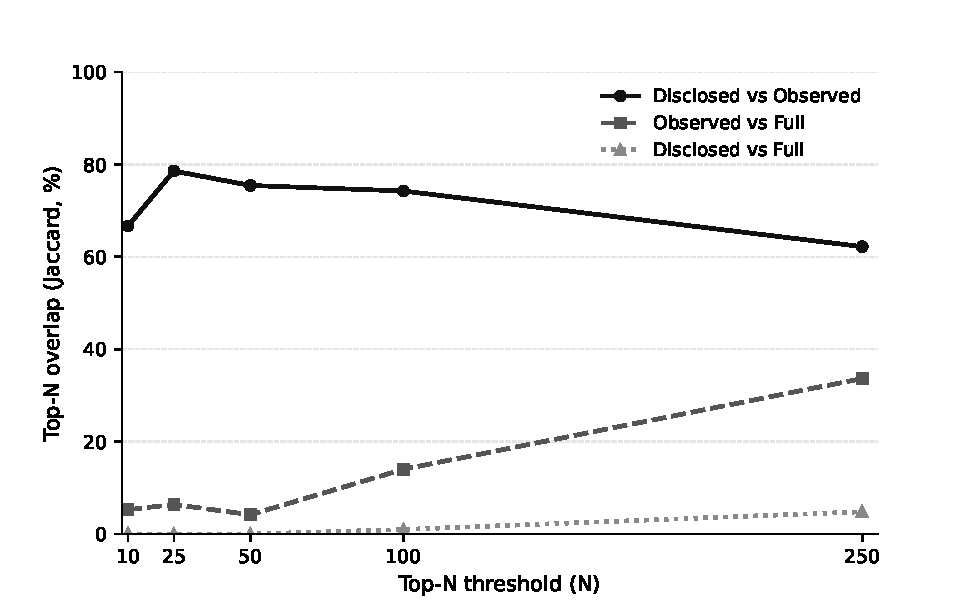
\includegraphics[width=\linewidth]{report/figures/fig_c_1_cross_view_overlap_curve.pdf}

  \captionsetup{justification=raggedright,singlelinecheck=false}
  \caption*{\footnotesize \textit{Note}. This figure reports pairwise Top-$N$ set overlap across evidence-conditioned views using Jaccard overlap (\%). For each view, the Top-$N$ set is constructed by ranking nodes by the same severity metric computed in that view and taking the first $N$ nodes. The disclosed--empirical curve reflects the empirically grounded stable core, while low empirical--augmented and disclosed--augmented overlap at small $N$ indicates top-tail sensitivity to predicted-layer expansion. See Table~\ref{tab:app_c1_crossview_stability_summary} for rank-correlation summaries.}
\end{figure}

%========================
% Appendix C.2
%========================
\section{Rank stability and confidence diagnostics (Table C.1)}
\label{app:c2_stability_confidence_diagnostics}

Table~\ref{tab:app_c1_crossview_stability_summary} complements the overlap curves with rank-stability diagnostics and confidence totals for high-impact candidates. The first block summarizes stability in the top tail. ``Top-25 overlap'' reports how many firms appear in both views' Top-25 lists, and the Jaccard overlap normalizes that intersection. ``Common ranked nodes'' is the number of firms that appear in both ranked lists and therefore can be compared directly. Spearman and Kendall correlations are computed on this common set and summarize whether two views preserve a similar ordering, even when Top-25 membership differs.

Two patterns matter for interpretation. First, adding shipping evidence refines but does not rewrite the highest-impact tail. Disclosed versus empirical has 22 of 25 overlapping Top-25 nodes (Jaccard 0.786). Ordering remains highly consistent on the common ranked set (Spearman 0.943, Kendall 0.867). Second, the augmented view materially reshapes the top tail relative to either evidence-grounded baseline. Empirical versus augmented overlap is low (3 of 25, Jaccard 0.064) and ordered agreement is weaker (Spearman 0.539, Kendall 0.597). Disclosed versus augmented shows no Top-25 overlap and little ordered agreement on the small set of nodes common to both rankings (Spearman $-0.119$, Kendall $-0.030$). This pattern is interpreted as evidence that predicted-layer visibility expansion can reorder which firms appear most consequential at the very top, even when the analysis objective is unchanged.

The second block reports confidence totals for the appendix high-impact candidate set using a tri-level cross-view presence rule. The high-impact set is defined as the union of candidates that fall within the pre-specified high-impact cutoff in any of the three evidence views. High confidence requires presence in all three views, Medium requires presence in two views, and Low indicates presence in one view. In the current build, this high-impact set contains 103 cases. None appear in all three views (High = 0). Forty-seven appear in two views (Medium = 47) and fifty-six appear in one view (Low = 56). These tiers are stability diagnostics. They are not probabilities, and they are not claims about the truth of any single supplier relationship. They also are not directly comparable to the confidence bins used in Figure~\ref{fig:ch4_action_matrix}, which apply a binary presence rule over a different cross-view candidate universe. Separately, Table~\ref{tab:ch4_strict_top25} reports a High/Medium/Low confidence label computed within the strict Top-25 shortlist, which combines the relevance filter with cross-view presence for decision reporting.

% ---------- Appendix Table C.1: Cross-view stability summary ----------
\begin{table}[tbp]
  \centering
  \caption[\textit{Cross-view stability summary across evidence views}]
  {\textit{Cross-view stability summary across evidence views}}
  \label{tab:app_c1_crossview_stability_summary}

  \footnotesize
  \setlength{\tabcolsep}{6pt}
  \renewcommand{\arraystretch}{1.04}

  % =======================
% Table C.1 (tabular only)
% Cross-view stability summary
% =======================
% chktex-file 1   user-defined macros in table cells terminated with space is correct
\begin{tabularx}{\textwidth}{@{}>{\raggedright\arraybackslash}X
  S[table-format=-2.3]
  S[table-format=-2.3]
  S[table-format=-2.3]
  S[table-format=3.0]@{}}
\toprule
Metric
& \multicolumn{1}{c}{Disc.\textendash Emp.}
& \multicolumn{1}{c}{Emp.\textendash Aug.}
& \multicolumn{1}{c}{Disc.\textendash Aug.}
& \multicolumn{1}{c}{Overall} \\
\midrule
\multicolumn{5}{@{}l}{\textit{Rank stability across evidence views}} \\
Top-25 overlap (count)         & 22    & 3     & 0     & \multicolumn{1}{c}{\textemdash} \\
Top-25 overlap (Jaccard)       & 0.786 & 0.064 & 0.000 & \multicolumn{1}{c}{\textemdash} \\
Common ranked nodes ($n$)      & 58    & 55    & 12    & \multicolumn{1}{c}{\textemdash} \\
Spearman rank correlation      & 0.943 & 0.539 & -0.119& \multicolumn{1}{c}{\textemdash} \\
Kendall rank correlation       & 0.867 & 0.597 & -0.030& \multicolumn{1}{c}{\textemdash} \\
\addlinespace[2pt]
\multicolumn{5}{@{}l}{\textit{High-impact set by confidence (integrated decision view)}} \\
High-impact, high confidence ($n$)   & \multicolumn{1}{c}{\textemdash} & \multicolumn{1}{c}{\textemdash} & \multicolumn{1}{c}{\textemdash} & 0   \\
High-impact, medium confidence ($n$) & \multicolumn{1}{c}{\textemdash} & \multicolumn{1}{c}{\textemdash} & \multicolumn{1}{c}{\textemdash} & 47  \\
High-impact, low confidence ($n$)    & \multicolumn{1}{c}{\textemdash} & \multicolumn{1}{c}{\textemdash} & \multicolumn{1}{c}{\textemdash} & 56  \\
High-impact total ($n$)              & \multicolumn{1}{c}{\textemdash} & \multicolumn{1}{c}{\textemdash} & \multicolumn{1}{c}{\textemdash} & 103 \\
\bottomrule
\end{tabularx}

  \captionsetup{justification=raggedright,singlelinecheck=false}
  \caption*{\footnotesize \textit{Note}. ``Disclosed'' uses disclosed SCR ties; ``Empirical'' adds observed shipping; ``Augmented'' adds the predicted-layer expansion used for sensitivity analysis. Top-25 overlap reports the intersection size and Jaccard overlap of the view-specific Top-25 ranked nodes under the section's severity metric. Rank correlations are computed on the set of nodes common to both views (``common ranked nodes''). Dashes indicate not applicable. The ``Overall'' column reports totals for the appendix high-impact candidate set by confidence tier, where confidence is defined by cross-view presence (High = present in all three views, Medium = present in two views, Low = present in one view). These confidence tiers are diagnostic and are not directly comparable to the binary confidence bins used in Figure~\ref{fig:ch4_action_matrix}, which are computed over a different candidate universe.}
\end{table}

%========================
% Appendix C.3
%========================
\section{Adjacent/Uncertain High-Impact Candidates}
\label{app:c3_adjacent_uncertain_validation}

This appendix section documents the \textit{adjacent/uncertain} reporting stream referenced in \S\ref{sec:ch4_decision}. The decision layer in Section~\ref{chap:network_analysis} is intentionally conservative. It promotes only those high-impact nodes that (i) are structurally consequential under the empirical evidence view and (ii) map cleanly to a semiconductor value-chain role under the strict relevance codebook. At the same time, a substantial set of nodes can remain highly consequential in the dependency fabric while being semantically ambiguous from an industry-code perspective. Rather than discarding these cases, they are retained as a structured validation queue to support auditability, adjudication, and future data enrichment.

Table~\ref{tab:app_c2_adjacent_uncertain_top25} reports the Top-25 adjacent/uncertain candidates under the empirical evidence view (disclosed SCR ties plus observed shipping), ranked by $H1_{\log}$. These rows use the same fixed severity estimates as the main analysis---counterfactual single-node removal evaluated on the locked empirical graph---but differ in reporting treatment. The industry-code basis is adjacent, coarse, or otherwise insufficient to support a defensible semiconductor value-chain role assignment. In practice, many high-impact adjacent/uncertain candidates cluster near primes (``Near-prime''), reflecting vendors and enabling services that sit one step upstream of DoD Tier-1 endpoints in the observed dependency fabric. This pattern is substantively important for decision use. It illustrates why raw disruption rankings must be filtered through a relevance and confidence layer before being described as semiconductor chokepoints.

Operationally, Table~\ref{tab:app_c2_adjacent_uncertain_top25} is used for \textit{validation}, not immediate prioritization as confirmed value-chain chokepoints. For each candidate, the appropriate next step is to adjudicate whether the observed dependency evidence plausibly represents semiconductor support (e.g., a material, equipment, packaging, or test dependency) versus an adjacent enablement relationship (e.g., enterprise software, IT services, facilities, or other generalized inputs) that is consequential for prime operations but not specific to semiconductor continuity. Candidates validated as semiconductor-relevant can be promoted via documented overrides or codebook refinement. Candidates that remain adjacent should be tracked separately as part of a broader operational-support risk posture. In either case, retaining this queue preserves transparency. It shows which structurally consequential nodes were deliberately \emph{not} promoted in the main-text chokepoint shortlist and why.

% -- Appendix Table C.2: High-impact adjacent/uncertain candidates (empirical) ----
\begin{table}[tbp]
  \centering
  \caption[\textit{High-impact adjacent or uncertain candidates (empirical view)}]
  {\textit{High-impact adjacent or uncertain candidates (empirical view)}}
  \label{tab:app_c2_adjacent_uncertain_top25}

  \footnotesize
  \setlength{\tabcolsep}{6pt}
  \renewcommand{\arraystretch}{1.04}

  % =======================
% Table C.2 (tabular only, appendix)
% Empirical Top-25 high-impact adjacent/uncertain candidates
% =======================
\begin{tabularx}{\textwidth}{@{}c
  >{\hsize=1.20\hsize\raggedright\arraybackslash}X
  >{\hsize=0.80\hsize\raggedright\arraybackslash}X
  c
  S[table-format=1.4]@{}}
\toprule
Rank & Firm & Code basis & Corridor & {$H1_{\log}$} \\
\midrule
1 & Microsoft & RBICS L2 5520 & Near-prime & 0.0093 \\
2 & JFrog & RBICS L2 5520 & Near-prime & 0.0063 \\
3 & MEDIA DO Co. & RBICS L2 5520 & Near-prime & 0.0062 \\
4 & Blackthorn.io & RBICS L2 5520 & Near-prime & 0.0038 \\
5 & 6Sense Insights & RBICS L2 5520 & Near-prime & 0.0038 \\
6 & Mediafly & RBICS L2 5520 & Near-prime & 0.0038 \\
7 & Zoom & RBICS L4 55153010 & Near-prime & 0.0036 \\
8 & Commerce.com & RBICS L2 5520 & Near-prime & 0.0030 \\
9 & Gogo & RBICS L2 6010 & Near-prime & 0.0029 \\
10 & Workday & RBICS L2 5520 & Near-prime & 0.0027 \\
11 & D2L & RBICS L2 5520 & Near-prime & 0.0025 \\
12 & DocuSign & RBICS L2 5520 & Near-prime & 0.0023 \\
13 & TeamViewer & RBICS L2 5520 & Near-prime & 0.0023 \\
14 & Top Group Software & RBICS L2 5520 & Corridor & 0.0023 \\
15 & Tufin Software Technologies & RBICS L2 5520 & Near-prime & 0.0023 \\
16 & Salesforce & RBICS L2 5520 & Near-prime & 0.0022 \\
17 & The Southern Co. & RBICS L2 6510 & Near-prime & 0.0022 \\
18 & Oglethorpe Power & RBICS L2 6510 & Near-prime & 0.0022 \\
19 & Unity Software & RBICS L2 5520 & Near-prime & 0.0022 \\
20 & Forescout Technologies & RBICS L2 5520 & Near-prime & 0.0020 \\
21 & SailPoint Technologies & RBICS L2 5520 & Near-prime & 0.0020 \\
22 & Perpetual Solutions & RBICS L2 5520 & Near-prime & 0.0019 \\
23 & DHI Group & RBICS L2 5520 & Near-prime & 0.0017 \\
24 & Ivanti Software & RBICS L2 5520 & Near-prime & 0.0017 \\
25 & Dayforce & RBICS L2 5520 & Near-prime & 0.0013 \\
\bottomrule
\end{tabularx}

  \captionsetup{justification=raggedright,singlelinecheck=false}
  \caption*{\footnotesize \textit{Note}. This table reports the 25 most structurally consequential nodes under the \textbf{empirical} evidence view (disclosed SCR ties plus observed shipping) that fall into the \textit{adjacent/uncertain} reporting stream under the semiconductor relevance procedure described in \S\ref{sec:ch4_decision}. Rows are ranked by $H1_{\log}$, the section's primary \textit{deny} severity metric: the log-obligation-weighted loss of semiconductor support to DoD Tier-1 prime endpoints under counterfactual single-node removal. ``Code basis'' reports the industry-code trigger (RBICS/SIC) responsible for classifying the firm as adjacent/uncertain rather than strict value-chain. ``Corridor'' indicates whether the node is embedded in the empirically supported semiconductor$\rightarrow$prime corridor; ``Near-prime'' indicates nodes one step upstream of primes within that corridor definition. Firm names omit corporate suffixes for readability. These entries are retained as a structured validation queue and are not promoted as decision-grade value-chain chokepoints (Table~\ref{tab:ch4_strict_top25}).}
\end{table}